\section{Infinity}

基于图像生成模型 VAR,Infinity 是对其进行优化而产生的文生图自回归模型。
VAR 采用传统的 index-wise 离散 tokenizer,受限于码本的词汇量大小,其面临着量化误差以及细节生成等问题,
尤其是对于产生高分辨率的图像,在生成阶段,它还面临着视觉细节丢失、局部扭曲、误差累计等问题。
针对这些问题,Infinity 进行了如下改进:
\begin{enumerate}
    \item \textbf{Bitwise visual tokenizer.} 采用 binary vector quantization 技术,将码本词汇量提升至
    $2^{64}$,因此显著提高了图像生成质量;
    \item \textbf{Bitwise infinite-vocabulary classfier.} 采用基于 binary bit 的分类预测,不同于传统的
    分类模型,在如此大码本下仍能保持高效的运算和优化;
    \item \textbf{Bitwise self-correction.} 在训练阶段随机 flip some bits 模拟预测错误,并重新量化残差特征,
    即随机引入预测误差,但在此误差下仍预测正确的残差特征,从而使模型获得自我纠正的能力。 
\end{enumerate}
Infinity 即是 bitwise VAR,它保持了 VAR 的 scaling 以及 speed 优势,同时也解决了 VAR 面临的问题,能够
实现高质量的图像生成效果,超过了 SD3-Medium 等扩散模型。

\subsection{Visual AutoRegressive Modeling}
Infinity 架构包括一个 visual tokenizer 以及 用于文生图的自回归 Transformer 模型,对于数据对
(prompt text $t$,image $I$),类似于 VAR, $I$ 首先被编码为特征 $F\in\mathbb{R}^{h\times w\times d}$,
然后量化得到 $K$ 个 multi-scale 残差特征 $(R_1, R_2, \cdots, R_K)$,定义
\begin{equation}
    F_k = \sum_{i=1}^{k} \text{upsample}(R_i,(h,w)),
\end{equation}
$F_k$ 逐渐逼近原始特征 $F$。自回归似然函数为
\begin{equation}
    P(R_1,\cdots,R_K) = \prod_{k=1}^K P(R_k|R_1,\cdots,R_{k-1},\Psi(t)),
\end{equation}
其中 $\Psi(t)$ 为基于 Flan-T5 模型的文本编码,在输入端,$\Psi(t)$ 首先被投影为一个 <SOS> token 作为第一步输入,
之后,每个 tranformer block,$\Psi(t)$ 还通过交叉注意力引导图像生成,在第 $k$ 步预测 $R_k$ 时,
$(\Psi(t),R_1,\cdots,R_{k-1})$ 作为输入,实际训练中,为匹配每一步输入输出端的分辨率大小,引入
\begin{equation}
    \tilde{F}_{k-1} = \text{downsample}(F_{k-1},(h_k,w_k)),
\end{equation}
作为输入去预测 $R_k$,故在第 $k$ 步预测中,实际的输入为 $(<SOS>,\tilde{F}_1,\cdots,\tilde{F}_{k-1})$,
$\tilde{F}_{k-1}$ 的分辨率大小与 $R_k$ 相同,在 VAR 中利用 $R_{k-1}$ 预测 $R_k$,输入时 $R_{k-1}$ 首先
经过了上采样以匹配 $R_k$ 的分辨率大小,相比之下 Infinity 处理方式更为恰当。

\begin{figure}[htbp]
    \centering 
    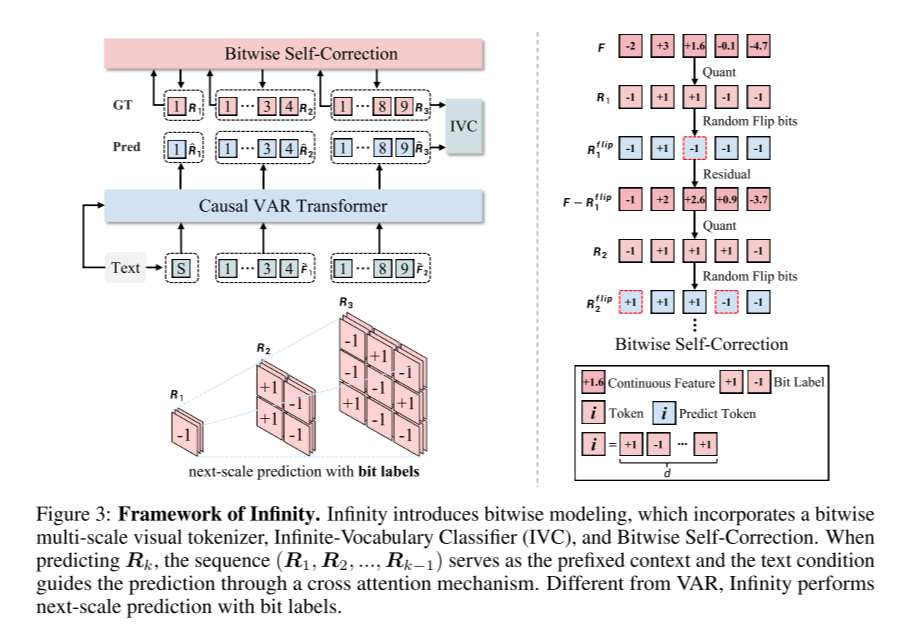
\includegraphics[width=0.8\textwidth]{./fig/Framework of Infinity.png} 
    %\caption{这是一张示例图片} 
    %\label{fig:example} 
\end{figure}

\subsection{Bitwise Visual Tokenizer}
增加码本的词汇量大小会显著增加存储和计算开销,为解决这个问题,Infinity 采用了 Bitwise multi-scale residual quantizer,
对每个尺度的特征向量 $z_k\in\mathbb{R}^d$,其被量化为 binary output $q_k$,
\begin{equation}
    q_k = Q(z_k) = \begin{cases}
        \text{sign}(z_k)\quad\text{if LFQ};\\
        \frac{1}{\sqrt{d}}\text{sign}(\frac{z_k}{|z_k|})\quad\text{if BSQ}.
    \end{cases}
\end{equation}
另外引入熵惩罚项 $\mathcal{L}_{\text{entropy}}=\mathbb{E}[H(q(z))]-H(\mathbb{E}[q(z)])$ 用于增加码本的利用率。

\subsection{Bitwise Infinite-Vocabulary Classifier}
由于码本词汇量巨大,在预测 $R_k$ 时,若采用原始的 softmax 分类器,会导致巨大的计算量,Infinity 采用 d 个二元分类器同时预测
$R_k$ 的每个 bit 是正还是负,从而大大提高效率和预测的鲁棒性。

\begin{figure}[htbp]
    \centering 
    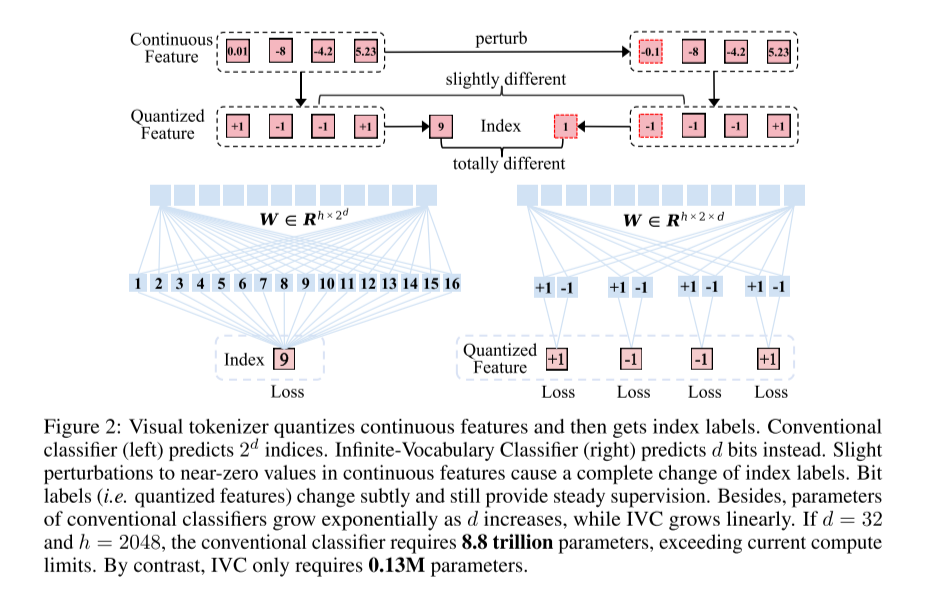
\includegraphics[width=0.8\textwidth]{./fig/IVC.png} 
    %\caption{这是一张示例图片} 
    %\label{fig:example} 
\end{figure}
\subsection{Bitwise Self-Correction}
在训练阶段,每一步的预测均是细化之前的输出,增加细节,但在实际生成过程中,若中间某一层出现预测误差时,模型
缺乏识别并修正错误的能力,从而导致误差累计。Infinity 根据一定概率随机 flip some bits 模拟预测错误,并重新量化残差特征,
这种引入过程错误,并根据错误调整预测目标使得模型具有识别并纠正错误的能力。

\begin{figure}[htbp]
    \centering
    \begin{minipage}{0.45\textwidth}
        \centering
        \begin{algorithm}[H]
            \caption{Visual Tokenizer Encoding}
            \begin{algorithmic}[1]
                \Require raw feature $F$, scale schedule $\{(h_1^r, w_1^r), ..., (h_K^r, w_K^r)\}$
                \State $R_{\text{queue}} = []$ \Comment{multi-scale bit labels}
                \State $\tilde{F}_{\text{queue}} = []$ \Comment{inputs for transformer}
                \For{$k = 1, 2, \cdots, K$}
                    \State $R_k = \mathcal{Q}(\text{down}(F - F_{k-1}, (h_k, w_k)))$
                    \State $\text{Queue\_Push}(R_{\text{queue}}, R_k)$
                    \State $F_k = \sum_{i=1}^{k} \text{up}(R_i, (h, w))$
                    \State $\tilde{F}_k = \text{down}(F_k, (h_{k+1}, w_{k+1}))$
                    \State $\text{Queue\_Push}(\tilde{F}_{\text{queue}}, \tilde{F}_k)$
                \EndFor
                \Ensure $\tilde{R}_{\text{queue}}, \tilde{F}_{\text{queue}}$
            \end{algorithmic}
        \end{algorithm}
    \end{minipage}\hfill
    \begin{minipage}{0.45\textwidth}
        \centering
        \begin{algorithm}[H]
            \caption{Encoding with BSC}
            \begin{algorithmic}[1]
                \Require raw feature $F$, random flip ratio $p$, scale schedule $\{(h_1^r, w_1^r), ..., (h_K^r, w_K^r)\}$
                \State $R_{\text{queue}} = [], \tilde{F}_{\text{queue}} = []$
                \For{$k = 1, 2, \cdots, K$}
                    \State $R_k = \mathcal{Q}(\text{down}(F - F_{k-1}^{\text{flip}}, (h_k, w_k)))$
                    \State $\text{Queue\_Push}(R_{\text{queue}}, R_k)$
                    \State $R_k^{\text{flip}} = \text{Random\_Flip}(R_k, p)$
                    \State $F_k^{\text{flip}} = \sum_{i=1}^{k} \text{up}(R_i^{\text{flip}}, (h, w))$
                    \State $\tilde{F}_k = \text{down}(F_k^{\text{flip}}, (h_{k+1}, w_{k+1}))$
                    \State $\text{Queue\_Push}(\tilde{F}_{\text{queue}}, \tilde{F}_k)$
                \EndFor
                \Ensure $R_{\text{queue}}, \tilde{F}_{\text{queue}}$
            \end{algorithmic}
        \end{algorithm}
    \end{minipage}
    \caption{Algorithms for Visual Tokenizer Encoding and Encoding with BSC}
\end{figure}